% Created 2020-07-07 mar 07:33
% Intended LaTeX compiler: pdflatex
\documentclass[letterpaper]{scrartcl}
\usepackage[utf8]{inputenc}
\usepackage[T1]{fontenc}
\usepackage{graphicx}
\usepackage{grffile}
\usepackage{longtable}
\usepackage{wrapfig}
\usepackage{rotating}
\usepackage[normalem]{ulem}
\usepackage{amsmath}
\usepackage{textcomp}
\usepackage{amssymb}
\usepackage{capt-of}
\usepackage{hyperref}
\usepackage{khpreamble}
\usepackage{subfigure}
\usepgfplotslibrary{groupplots}
\addtolength{\oddsidemargin}{-4mm}
\addtolength{\evensidemargin}{-4mm}
\addtolength{\textheight}{33mm}
\author{Kjartan Halvorsen}
\date{}
\title{}
\hypersetup{
 pdfauthor={Kjartan Halvorsen},
 pdftitle={},
 pdfkeywords={},
 pdfsubject={},
 pdfcreator={Emacs 26.3 (Org mode 9.3.6)}, 
 pdflang={English}}
\begin{document}



\section*{Bode- and Nyquist plots, relative stability}
\label{sec:org208b430}
Kjartan Halvorsen, September 2019

Sketch the Nyquist plot corresponding to the Bode plot! Then mark the phase margin and amplitude margins!
\begin{center}
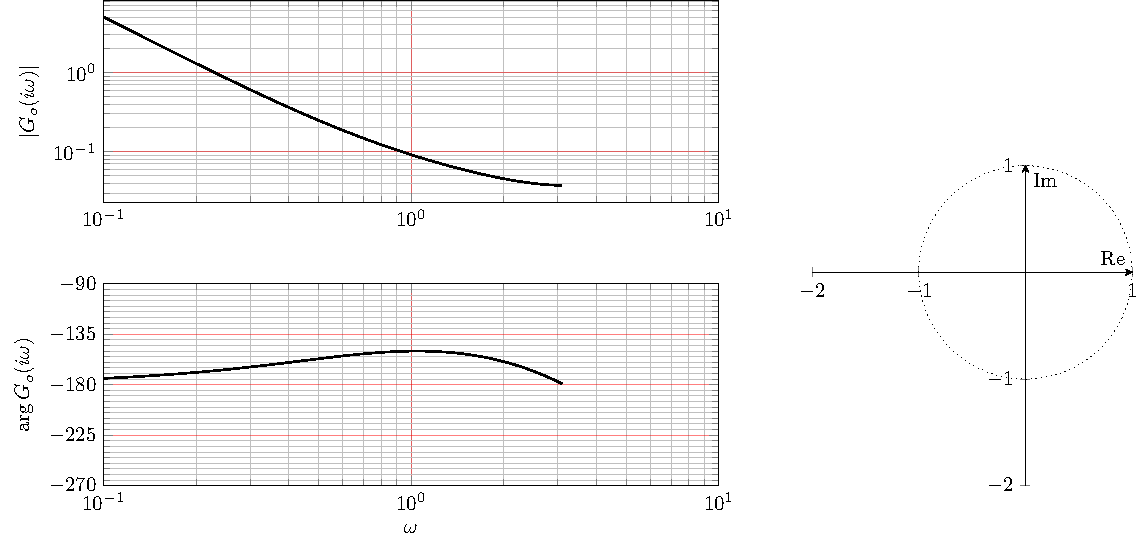
\includegraphics[width=1.15\linewidth]{../../figures/bode-nyquist-exc-1}
\end{center}

\begin{center}
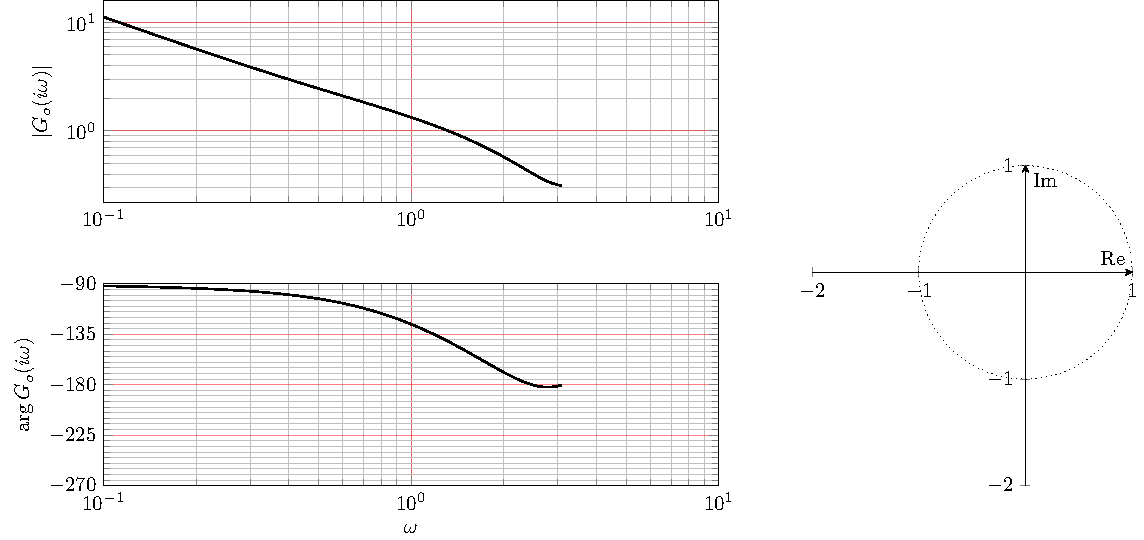
\includegraphics[width=1.15\linewidth]{../../figures/bode-nyquist-exc-2}
\end{center}
\end{document}